\begin{question}
\noindent A UI/UX designer is prototyping a symmetrical icon on a grid-based design canvas. She has drawn triangle $T$ and wants to check the mirror-image icon by reflecting it in the vertical line $x = 2$.

\begin{center}
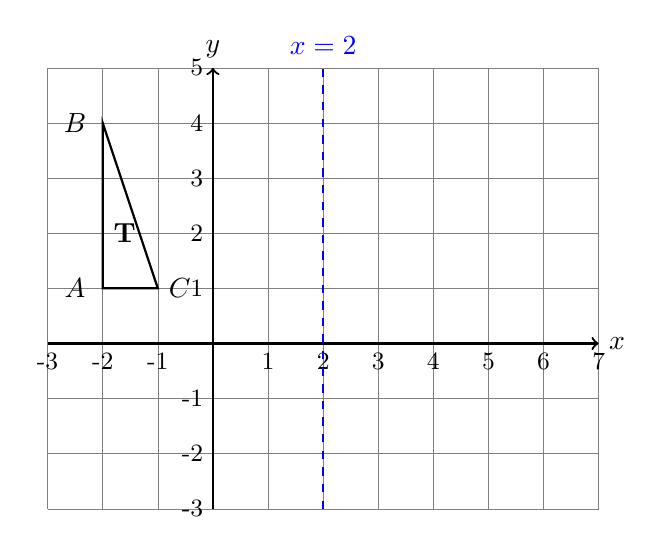
\begin{tikzpicture}[scale=0.7]
    % Grid
    \draw[step=1cm, gray, very thin] (-3,-3) grid (7,5);

    % Axes
    \draw[thick,->] (-3,0) -- (7,0) node[right] {$x$};
    \draw[thick,->] (0,-3) -- (0,5) node[above] {$y$};

    % axis numbers
    \foreach \x in {-3,-2,-1,1,2,3,4,5,6,7}
        \node[below] at (\x,0) {\small \x};
    \foreach \y in {-3,-2,-1,1,2,3,4,5}
        \node[left] at (0,\y) {\small \y};

    % Mirror line x=2
    \draw[thick, dashed, blue] (2,-3) -- (2,5);
    \node[blue] at (2,5.4) {$x=2$};

    % Triangle T
    \draw[thick] (-2,1) -- (-2,4) -- (-1,1) -- cycle;
    \node at (-2.5,1) {$A$};
    \node at (-2.5,4) {$B$};
    \node at (-0.6,1) {$C$};
    \node at (-1.6,2) {\textbf{T}};

\end{tikzpicture}
\end{center}

\noindent Triangle $T$ has vertices $A(-2,1)$, $B(-2,4)$ and $C(-1,1)$.

\noindent Reflect triangle $T$ in the line $x = 2$.

\vspace{4cm}

\begin{flushright}
    \answerplain{2}
\end{flushright}
\end{question}